% easychair.tex,v 3.5 2017/03/15

\documentclass{easychair}


\usepackage{doc}
%
\newcommand{\easychair}{\textsf{easychair}}
\newcommand{\miktex}{MiK{\TeX}}
\newcommand{\texniccenter}{{\TeX}nicCenter}
\newcommand{\makefile}{\texttt{Makefile}}
\newcommand{\latexeditor}{LEd}

%\makeindex

%% Front Matter
%%
% Regular title as in the article class.
%
\title{An automatic on-chain verification of Java smart contracts}

\author{
Luca Olivieri\inst{1,2}
\and
Fausto Spoto\inst{1}
\and
Fabio Tagliaferro\inst{1}
}

\institute{
  Università degli Studi di Verona, Italy\\
  \email{\{luca.olivieri, fausto.spoto, fabio.tagliaferro\}@univr.it}
\and
   Corvallis S.r.l., Padova, Italy\\
 }

\authorrunning{L. Olivieri, F. Spoto, F. Tagliaferro}

\titlerunning{An automatic on-chain verification of Java smart contracts}

\begin{document}

\maketitle

\begin{abstract}
  Blockchain protocols allow the programming of smart contracts: computer code handling and expressing agreements among parties.
  The distributed execution of contracts is enforced by a consensus protocol, as a consequence of transactions signed and broadcasted by the users of a blockchain network.
  Smart contracts are typically written in a high-level programming language and once deployed/installed in blockchain they become practically immutable.
  This immutability feature, achieved through a cryptogra\-phically-linked chain of blocks and a consensus algorithm, guarantees code integrity and avoids tampering by third parties.
  Bugs in smart contract code have dangerous consequences (such as rule violations and security attacks) causing economic losses.
  Indeed, immutable contracts can lead to immutable bugs that cannot be easily patched.
  For this reason the correctness of smart contract code must be ensured, for example with verification techniques.
  Typically, developers should check the code with verification tools (\emph{e.g.}, \cite{TIGR21, GriecoSCFG20, FeistGG19}) on their machine or by leveraging third-party services (\emph{i.e.}, outside of blockchain and hence \emph{off-chain}), before smart contract installation.
  However, this approach is \emph{optional}: naive programming without verification could still occur and none of the existing blockchain protocols force its use at all.
  Instead, an automatic \emph{on-chain} verification occurs among the nodes of a blockchain network, as part of its consensus rules.
  On-chain smart contract verification acts as a \emph{mandatory} filter that blocks the installation of code that does not abide to the verification rules, effectively making their execution impossible.
  The verification module should be efficient (the network should not be burden by the distibuted verification) and deterministic (every node should have the same result to achieve result).
  These requirements make the development of an on-chain solution a challenging task.
  In addition, it needs a specific technique for updating the consensus rules of a network after a change of the verification rules.
  The re-verification of previously installed smart contracts (with the latest verification checks) must be enforced too, assuring that every smart contract has been verified with the latest checks before being executed.
  We implemented a on-chain smart contract verification solution for the Takamaka subset of Java~\cite{Spoto19} as a decentralized application in a Proof-of-Stake (PoS) blockchain exploiting Tendermint Core~\cite{tendermintcore}, as shown in fig.~\ref{fig:architecture}.
  Our verification module includes $26$ on-chain checks verifying the correct use of Takamaka's primitives and code annotations while only allowing the use of a
  deterministic subset of the Java library~\cite{Spoto20}.
  In our implementation, the verification module can be upgraded only with network consensus, as a result of a successful poll proposed and voted by stakeholders through a Takamaka smart contract.
  Conceptually, an update of the verification module requires the re-verification of all code already installed in blockchain.
  This procedure could be really expensive since it would hang the nodes for a long time.
  However, the experience on the popular and public blockchain Ethereum~\cite{Buterin13} is that only $0.05\%$ of all contracts installed are involved in $80\%$ of the transactions~\cite{OlivaHJ20}, suggesting that a complete re-verification of the installed smart contracts could be a waste of time.
  For this reason, our solution is to lazily re-verify the code only on-demand, when it is asked to run.
  A lazy approach amortizes the costs of an update to the verification module by avoiding the re-verification of code that might actually never run again.
  Finally, once that a smart contract has been blocked by re-verification it won't be possible to restore it.
  We evaluated the scalability of our technique with a smart contract that creates and funds a pool of $500$ externally-owned accounts and allows one to determine which is the \emph{richest} among them (has highest balance).
  Our experiment installs that smart contract in blockchain and uses it to create and fund the $500$ accounts, execute $1,000$ random money transfers between them and asks for the richest.
  The difference between the experiment performed with/without on-chain verification was only $0.79\%$ in terms of transactions per second.
\end{abstract}

\begin{figure}[t]
  \begin{center}
    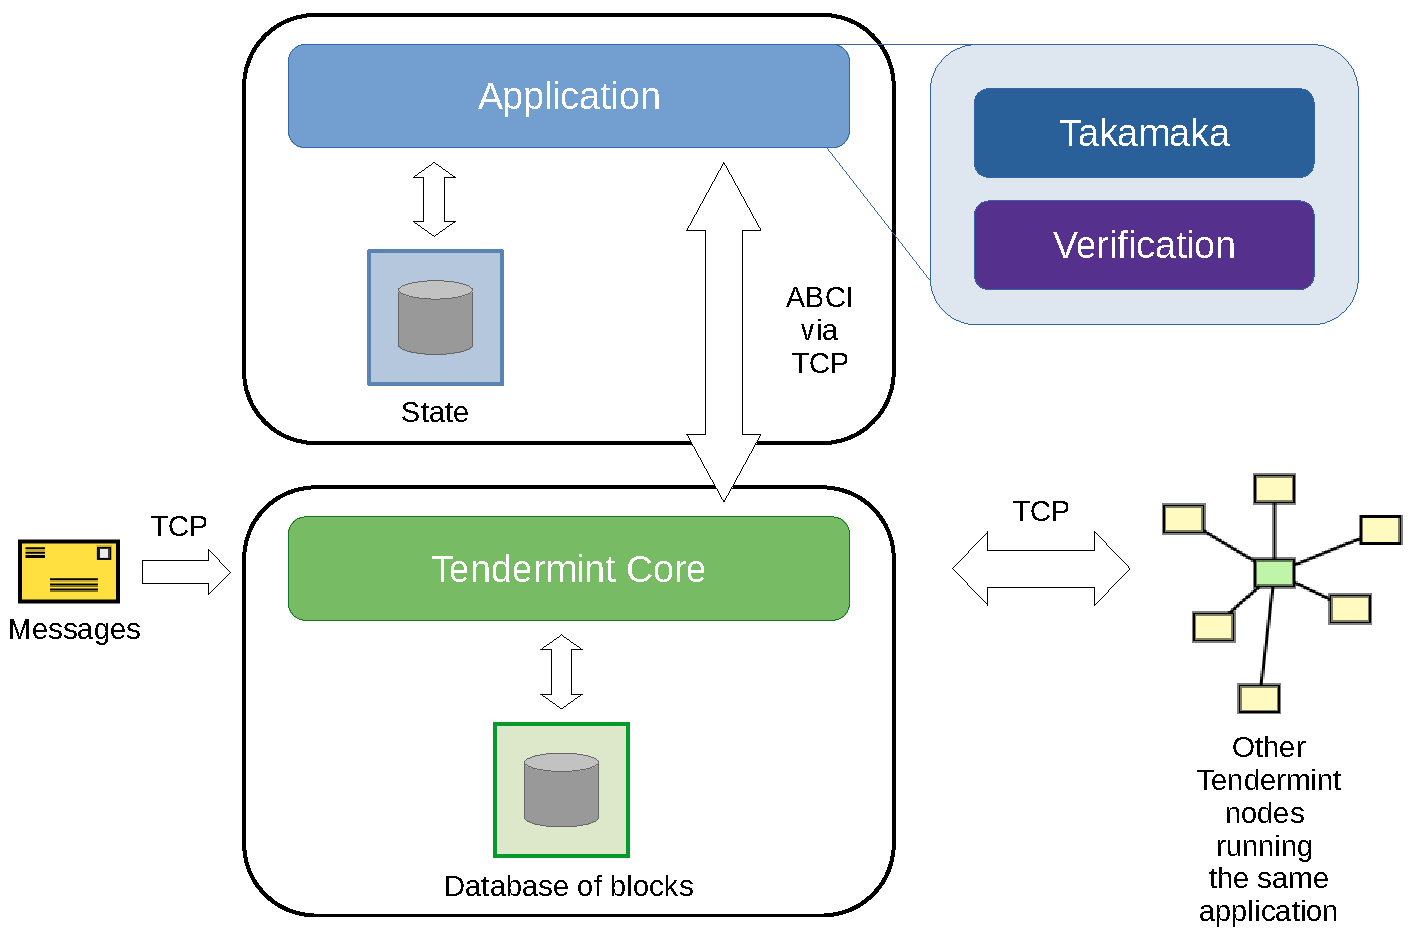
\includegraphics[scale=0.4]{pictures/architecture.pdf}
  \end{center}
  \caption{Architecture of our distributed application performing on-chain verification.}
  \label{fig:architecture}
\end{figure}

\bibliographystyle{plain}
\bibliography{biblio}

\end{document}
